\section{Software Tool Internals}
\label{SoftwareToolInternals}

In the software tool, the constellation is simulated, and the inverse problems of the altitude and BRDF determination are solved. For the simulation of the constellation, the satellites were given a set of parameters. Furthermore, every satellite has a set of Keplerian elements which provide the orbit. 

For the main emitter satellite there are a few other parameters describing the laser behavior. These are the laser wavelength, the beam divergence, the pulse time and the power. The power is the actual lasing power of the laser, so not the input electrical power of the laser. Note that the laser is perpetually nadir-pointing.

For the receiving satellites, the receiver is characterized by the receiver spectral filter width, the aperture area, the receiver beam divergence (which determines the footprint) and the receiver efficiency. The receiver efficiency is composed out of the optical efficiency ($\sim0.9$) and receiver chip efficiency ($\sim0.34$). Note the receiver is assumed to be perfectly pointed to the emitter footprint. Also, the footprint of the receiver is larger than the footprint of the emitter.

The basic path of the signal is as follows: First it is transmitted, then it propagates downwards through the atmosphere to the earth. There it scatters back in all directions. If there is sunlight shining on the footprint, that is also scattered upwards. In the direction of each receiving satellite, a small cone of the reflected energy is scattered. This again propagates through the atmosphere and is then received by the receivers. The internals of the simulation steps will be discussed more closely in the following sections.


\subsection{Signal Emmission}
As mentioned before, the signal is emitted at the position of the emitter satellite. The power in each pulse can be determined by spreading the continuous lasing power of the laser over its duty cycle:

\begin{equation}
	P_{pulsed} =  \frac{P_{continues}}{pulse length \times pulse frequency}
\end{equation}

This means that the power in each pulse is high compared to the continuous lasing power. The pulse is directed towards the satellite nadir. This means that when the signal travels trough the atmosphere it encounters an airmass of exactly one.

\subsection{Atmospheric effects}

When a signal travels through the atmosphere, it is modified in several ways. Of these modifications, the largest effect is the atmospheric attenuation of the signal. This is also the only type of atmospheric effect that is taken into account.

The atmospheric attenuation is dependent on both optical thickness of the atmosphere and airmass (path length through the atmosphere). The airmass factor can be found using equation \ref{eq:airmass}. The optical thickness is dependent on the laser frequency and can be found in tables (for 473 nm this is about 10\%). The attenuation of the signal can then be computed with equation \ref{eq:AtmAttenuation}.

\begin{equation}
	l = sec (z)
	\label{eq:airmass}
\end{equation}
\begin{equation}
	I = I_0 \: e^{ -optThick \cdot l }
	\label{eq:AtmAttenuation}
\end{equation}

In equation \ref{eq:airmass}, $z$ is the zenith angle (angle between the satellite direction and up direction on the earth). Note this equation is only valid when the satellite is not near the horizon, because then this formula breaks down. However, due to the maximum angular separation of 2.18$^\circ$ this situation is not encountered.

\subsection{Scattering}
\subsubsection{Laser Scattering}
\label{scatter}
When the laser pulse reaches the ground it is scattered back. The scattering model used to describe this is taken from the discussion thereon in \cite{rees}. 

Scatter is the physical process where incident radiation is absorbed and reflected back towards the atmosphere. To this end a scattering model is used. This scattering model is a way to construct a \ac{BRDF}. A \ac{BRDF} is a distribution of the incident light over the hemisphere \cite[pages 47-49]{rees}. An example is shown in figure \ref{fig:scatter}, page \pageref{fig:scatter}.\\\\
The most basic example of a \ac{BRDF} is the Lambertian model \cite[pages 49-50]{rees}. This model assumes a homogeneous perfectly rough surface, causing a homogeneous scattering distribution. Apart from the index of refraction of the air, the incident radiation vector and the exittant radiation vector (which are all known), use of Snell's law is needed to find Fresnel's coefficients, thereby requiring the index of refraction of the ground. Due to the complexity of the algebraic equations in computing the Lambertian coefficient, a set of a hundred points where evaluated in Mathematica. Through these points, a 4th order polynomial was fitted. This polynomial is then evaluated at the given material index of reflection to give the Lambertian constant.

A modification that can be made to take into account the tendency of surfaces to scatter more in the direction of the surface normal, is called the Minnaert model \cite[page 50]{rees}. It causes a more elliptical \ac{BRDF}. It depends on the Minnaert parameter $\kappa$.

Another important modification is the Henyey-Greenstein term. It accounts for the tendency of surfaces to back- or forwardscatter \cite[page 51]{rees}. This rotates and deforms the elliptical \ac{BRDF} obtained from the Minnaert model. The Henyey-Greenstein term is parameterized by $\Theta$. The final result is shown in figure \ref{fig:scatter}, page \pageref{fig:scatter}.\\\\
This is the scattering model used in the program. Because there is no data from which all three parameters can be accurately determined, a coefficient map was made up. It does not matter much what the precise form of the \ac{BRDF} used in the simulation is, so long as it can be retrieved.

With the help of the formulae from \cite[pages 43-51]{rees}, the incidence vector can be taken and the number of photons radiated in a specific direction can be calculated. This is done by the same algorithms both for laser photons a for sun noise.

\begin{figure}[ht!]
\centering
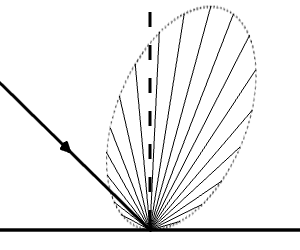
\includegraphics[width=0.4\textwidth]{chapters/img/scatter.png}
\caption{Example of a \ac{BRDF}}
\label{fig:scatter}
\end{figure}

\subsubsection{Noise Scattering}
Also noise is reflected up to the satellites. This reflection takes place in the receiver footprint. Because the direction of the receiver is not perpendicular to the normal of the reflection area, the footprint becomes elliptical. Over this entire elliptical area, solar radiation is reflected to the receiver. The semi major and minor axis of this ellipse can be computed based on divergence of the sensor beam (receiver beam divergence). The \ac{SPAD} multi pixel behavior is not implemented in the software, because this change would lead to the software not being completed in time. In order to approximate its behavior on a noise level, only the set of pixels that look directly to the emitter footprint are therefore bundled into one equivalent footprint. 

The amount of solar flux that is reflected up to the satellites is only the flux in the spectral width of the receiver. Then using the laws of gray body radiation, the amount of solar flux inside the receiver footprint in the given spectrum is computed. The equation used to compute the influx is:

\begin{equation}
	\lambda_{1,2} = \lambda _{laser} \pm \frac{Wavelength Bandwidth}{2}
\end{equation}
\begin{equation}
	I = \sigma T^4 (f(\lambda _1, T, \epsilon) - f(\lambda _1, T, \epsilon))
\end{equation}

In this equation $f(x)$ is an approximation of Planck's Integral \cite[p.~26]{rees}. This flux is then scatted in the same manner as for the laser scattering, to all the receivers. The big difference is that this is a continuous process, whereas the laser scattering happens in discrete steps.

\subsection{Reception by the receiver}
When the the energy of the laser pulse and the noise, reach the receiver again, the amount of received photons can be determined. This is done based on the energy per photon, which is defined in equation \ref{eq:PhotonEnergy}. Now the total number of received photons is equal to the inbound energy divided by the energy per photon. The floating point remainder is then compared to a random generated number from zero to one, and if the random number is smaller than the remainder, an extra photon is added.

\begin{equation}
	E_{p}=\frac{h \cdot c}{\lambda}
	\label{eq:PhotonEnergy}
\end{equation}

In equation \ref{eq:PhotonEnergy}, $h$ is the Planck constant, $c$ the speed of light and $\lambda$ the wavelength of the emitter laser (473 nm).

\subsection{Orbit}
\label{orbit}
The orbit of each satellite in the constellation is defined by means of six Keplerian elements. These define the shape of the orbit, the orientation of the orbit with respect to the center of the Earth and the position of the satellite on the orbit.\\\\
As there are a number of rotating bodies, three reference frames are used in order to facilitate the process of locating the satellites in space. The three reference frames used in the simulation are described below.

The first is the \ac{TOD} frame, and it is a more precise implementation of the \acs{ECI} frame. Its X-axis points towards the direction of the vernal equinox and its Z-axis coincides with the axis of rotation of the earth. \ac{TOD} takes into account nutation and precession of the earth. For practical reasons, it does not rotate with respect to the Sun.
 
In the second place there is \ac{ECEF}. Its X-axis points towards $0^\circ$ latitude and $0^\circ$ longitude. The XY plane lies in the plane of the equator. Its origin is in the center of mass of the Earth. 

Thirdly there is the PQW. The P-axis points towards the perigee of the orbit, the PQ plane lies in the plane of the orbit and the W-axis is perpendicular to the plain of the orbit. The origin of the frame is at the focal point. 

The program converts between the before-mentioned reference frames for the user's convenience.\\\\
The position of the satellite is defined with respect to the \acs{TOD} reference frame. Kepler's equations are solved for a certain time to determine the position. The orbit is determined for every satellite in the constellation. The orbit is assumed to be perfect, meaning that its orientation and shape do not change: perturbations are not considered. 

The Earth's rotation about its own axis and around the Sun is simulated in order to provide a more realistic simulation environment. From the rotation of the Earth around the Sun, the sun vector is deduced; this is used in noise calculations.

Most of the functions are adapted to the simulator from the \ac{JAT} library. 